
\documentclass[12pt]{article} % use larger type; default would be 10pt

\usepackage[utf8]{inputenc} % set input encoding (not needed with XeLaTeX)

\usepackage{geometry} % to change the page dimensions
\geometry{a4paper} % or letterpaper (US) or a5paper or....

\usepackage{graphicx} % support the \includegraphics command and options

\usepackage{booktabs} % for much better looking tables
\usepackage{array} % for better arrays (eg matrices) in maths
\usepackage{paralist} % very flexible & customisable lists (eg. enumerate/itemize, etc.)
\usepackage{verbatim} % adds environment for commenting out blocks of text & for better verbatim
\usepackage{subfig} % make it possible to include more than one captioned figure/table in a single float
\usepackage{braket}
\usepackage{mdframed}
\usepackage[toc,page]{appendix}
\usepackage{setspace}

\usepackage{caption}
\usepackage{pdflscape}

%\usepackage{subcaption}

\widowpenalty10000
\clubpenalty10000


%%% SECTION TITLE APPEARANCE
\usepackage{sectsty}
\allsectionsfont{\sffamily\mdseries\scshape} % (See the fntguide.pdf for font help)
% (This matches ConTeXt defaults)

%%% ToC (table of contents) APPEARANCE
\usepackage[notlof,notlot]{tocbibind} % Put the bibliography in the ToC
\usepackage[titles,subfigure]{tocloft} % Alter the style of the Table of Contents
\renewcommand{\cftsecfont}{\sffamily\mdseries\upshape}
\renewcommand{\cftsecpagefont}{\sffamily\mdseries\upshape} % No bold!

%\usepackage{titlesec}
%\titleclass{\section}{top}
%\newcommand\sectionbreak{\clearpage}

\let\oldsection\section
\renewcommand\section{\clearpage\oldsection}

\usepackage{enumitem}
\setlist{nolistsep}
\renewcommand{\descriptionlabel}[1]{\hspace{\labelsep}{\scshape #1}: }

\usepackage{amsmath}
\usepackage{amssymb}
\usepackage{changepage}

\usepackage{hyperref}
\hypersetup{
    colorlinks=true, %set true if you want colored links
    linktoc=all,     %set to all if you want both sections and subsections linked
    linkcolor=blue,  %choose some color if you want links to stand out
    linktocpage
}

\renewcommand{\familydefault}{\sfdefault}



\begin{document}
\begin{titlepage}


    \centering

    \vspace*{4cm}
  {\scshape\huge Tembryo: 18 Month Roadmap}\\
  
	 %\includegraphics[width=0.4\columnwidth]{oxford_crest.eps}\\
\vspace*{\fill}
	 {\scshape\huge\Large Private and Confidential\\
	 August 2016}

\end{titlepage}


\tableofcontents{}


\doublespacing
\setlength{\parindent}{0pt}
\setlength{\parskip}{0.7\baselineskip}%

\section{Introduction}

Our objective over the next 18 months is to build a compelling AI coaching product for a single game (Dota 2) and position ourselves to raise a Series A so that we can expand into multiple eSports. This report outlines our strategy for getting there and includes:
\begin{itemize}  
\item Funding: How much funding we need and how it will be used
\item Product: The stages of development for the product 
\item Technical: Supporting material on system architecture
\item Team: Who we need to hire
\item Timeline: How the product and team fit together to achieve the required milestones.
\item Market: Analysis of existing products and competitors
\end{itemize}

\section{Funding}

A seed round of \pounds350k will support a team of 2 founders, a front-end engineer, a back-end engineer and a marketing manager for 18 months. This gives sufficient time to build the features required to start generating revenue and begin to estimate important parameters for the business model, such as the conversion rate to paying customers, churn rate and cost of acquisition.

The funding will be used as follows:

\begin{itemize}
\item \pounds240k on Salaries (70\%):
\begin{itemize}
\item 2 x Founders: each \pounds25k per year
\item Front-end Developer: \pounds40k per year
\item Back-end Developer: \pounds40k per year
\item Marketing Manager: \pounds30k per year 
\end{itemize}
\item \pounds36k on Office Rent (10\%)
\item \pounds15k on Marketing (4\%)
\item \pounds25k on Server Costs (6\%)
\item \pounds35k Reserved (10\%)
\end{itemize}

\section{Product}

The table below sets out the planned three phases of product development. In each phase all users will be given access to some portion of new features for free, whilst the rest are reserved for paying subscribers. In the rest of this subsection we describe the features in more detail, and in the next section we give an overview of the involved technology.

\begin{center}
\onehalfspacing
    \begin{tabular}{ | l | p{6cm} | p{6cm} |}
    \hline
    Phase & Features  & User Perspective\\ \hline
    Current & A neural network that provides ratings for multiple attributes/skills and simple tips on how to improve.
 &``Allows me to see long-term trends in my play and ideas on how to improve as a player''\\  \hline
    Phase 1 & Automatic match parsing, event evaluation using statistics from the replay file dataset. AI tips for specific situations (e.g., ward placement)
 & ``A vital tool for highlighting particular mistakes in my past matches. I get information that I just can`t get anywhere else'' \\ \hline
    Phase 2 & AI for that provides suggestions of optimal actions and strategies alongside the match review.  & ``A tool that understands the game shows me what I need to focus on if I want to improve. I get presented alternative strategies and see how I could have done better.''  \\
    \hline
     Phase 3 & Rendered video content synchronized with coaching suggestions. Library of video content for helping players improve. & ``I get important game situations presented just as they are in game, which helps me visualise what I`m supposed to do next time I play.'' \\
    \hline
    \end{tabular}
\end{center}
\pagebreak

\subsection{Current State}

The prototype website currently consists of 2 main features: a performance rating feature and a match review feature.

The performance rating feature solves a problem with the current player rating system provided by the game developers. In Dota 2, each player is given a MMR (Match Making Ranking), which is a single number that ranks their skill level using the same method as an Elo score in chess. Rankings such as MMR are a feature that is common to all eSports because developers need a method of matching up similarly skilled player to create evenly matched teams. The problem is that because MMR is the aggregation of all the win/loss outcomes over your career as a player it does not give any information about your performance in a particular match. This limitation of the MMR in Dota 2 has been a topic of discussion amongst players on forums and is frequently cited by our users as one of the things they like best about the page.

The second main feature is the match review page. When a player selects one of their matches from their match list, we provide a simple animation of the match that shows the ten players moving around the game map. At present this visualisation provides limited information to the user: timing of kills, timing of fights, where `creep' deaths occur, but users report that they find it useful for reminding themselves what happened in a match.

\subsection{Phase 1} 

In Phase 1 (first 6 months) we will further develop our event based summary of matches i.e., a segmentation of the match into a sequence of events that capture at a high level what is happening in the match at each point in time. For example, an event in a Dota 2 match might be ``farming creeps'', or ``attacking opponents tower''. These events will be displayed on the visualisation of the match along with a text summary containing information relevant to the event. For example for a ``farming creeps'' event the text will display information such as the number of last hits achieved or the amount of gold earned. The event summary will eventually form a crucial component in the automated coaching features that come in subsequent phases, and so the design of the user interface will need to be tested carefully with users to ensure that it is intuitive to use.

We will leverage our replay file dataset to provide statistics on how well the players performed at each event compared to other players. Returning to the `creep farming' example, we will provide stats on how efficiently the player farmed i.e., you were in top 25\% of players for gold per minute farmed for this period of the match. The events in the visualisation will be colour coded according to how well they performed to help them focus on particular events where they perform less well.

We will also use the dataset we have collected to construct models of isolated parts of the game mechanics, and use Artificial Intelligence approaches, such as action planning or genetic algorithms, to compute alternative sequences of actions that a player could take in order to improve their play. As an example use case, this approach will allow us to suggest precise sequences of hero abilities that a player could use in order to reduce the amount of time it takes them to achieve certain objectives within the game such as `farming". This is a level of feedback that far exceeds anything that is currently available for eSports players and should be a tipping point where our conversion rate from free to paid users improves to between 2-5\%.

\subsection{Phase 2}

In Phase 2 (6th to 12th month) we will advance the Artificial Intelligence technology to move from optimisation of specific subproblems, which are picked using human knowledge about the game, towards a system that analyses the game as a whole. Combining the methods developed in Phase 1 with ideas from reinforcement learning and machine learning will result in a system that relates situations and actions to the outcome of the game. This will improve the coaching capabilities and should evene allow the Artificial Intelligence to discover options overlooked by expert players. A predecessor with similar algorithmic ideas is AlphaGO, a recent milestone of AI technology developed by Deep Mind, which was the first program to beat a world-class human player in the game of Go.

Driven by the Artificial Intelligence system, we will generate an evaluation of gameplay to the users that actually tells them precisely what leads them to winning or losing matches. From here we will support users in picking personalised performance metrics to guide their improvement. For example, a user might wish to focus on improving their last hitting performance, because mistakes in this kind of situation get highlighted by the system as particularly important. From here we provide an interface for them to set targets for the average percentage of last hits achieved. We will then track their performance in subsequence matches and send a weekly, personalised report on summarising how well they performed, along with links to articles and video content on improving that aspect of their game.

\subsection{Phase 3}

In Phase 3 (12th to 18th month) we will generate short video clips of the user playing by rendering videos using the game client. This will require us to build the infrastructure to host the game client software in the cloud, load a specific replay file, and then grab frames from the screen to make generate a video. This video would then also be need to compressed before being displayed in the user's browser. The value of rendering video is that it helps the user visualise their mistakes as the coaching is presented in a form closer to what they actually experience whilst playing the games. By combining the information extracted from the replay files and the rendered videos we can also build other features such as automatic highlight reels for users to share with their friends.

\section{Technical}

Realising the goal of an engaging web application that provides automated coaching to millions of players requires the development of a diverse mix of software that has to be highly scalable. We employ a service oriented architecture, splitting the the different tasks that have to be performed in the backend into multiple small programs that perform very specific tasks. This allows individual scaling of the software, depending on load and computational requirements. Another benefit is isolation of development, letting us implement and update different parts of the software with clear system boundaries.

For example, match analysis takes considerably more time than match download. As compensation we might run ten times more instances of the Analysis service than the Download service. The Analysis service might also be written in a different language than the Download service, use some machine learning libraries, and be modified a lot more frequently. Due to the isolated architecture a developer can work on the Analysis service without knowing anything about other services.

\subsection{Hosting}

The server software runs on common virtual servers, which are available from a multitude of hosting providers. Dependencies on specific providers are avoided or kept to a minimum, as we want to first use available hosting credit from multiple partnership programs and later on freely pick providers based on price. The current setup runs on machines provided by DigitalOcean, while using Google Cloud Platform to store the sizeable amount of replay files necessary as training data. In the next step we will move all hosting to Google Cloud Platform in order to use \$20k in hosting credits made available by Y-Combinator. 

\subsection{Deployment/Orchestration}

All backend software is containerised using Docker to specify the full environment of a program at development. Each service runs in a separate container, and services can be scaled up by deploying multiple instances of the same container. The instances are distributed over the pool of available servers, communicating over a central message passing system and sharing data in the main database.

Currently the set of servers is small enough to manage the container instances by hand. In the next step, we will integrate Docker Swarm to ease the orchestration and prepare for further scaling. Later on we will add additional systems to monitor system load and automatically adjust the available computational capacity.

\subsection{Backend}

The backend consists of multiple services performing different jobs using various different technologies. The database service stores all persistent structured data. Currently we use the proven open-source database PostgreSQL. To prepare this system for further growth, we will evaluate the available options and either scale the database using the sharding extension Citrus, or switch to an inherently distributed database like Kassandra.

Currently communication between services is performed over the notification feature of the PostgreSQL database. Further into development this will be moved out into a specialised system, possibly using the open-source message broker RabbitMQ.

The website is served by a nginx instance, to allowing for HTTP load balancing. The webserver itself is implemented in Javascript using Node.js/Express, with data for the interactive elements of the webpage exposed through a REST API. In another development step we will move the data transfer to websockets, which will improve efficiency, responsiveness, and separation between static web pages and data API.

Most server process logic is implemented using Javascript/Node.js, an accessible setup for new backend developers with a large available ecosystem of software packages. Examples for this are the Retrieve service, which handles the connection to the Steam network to access match data, and the Download service that pulls replay files from Steam servers and adds them to our dataset.

The Analysis service is mostly written in other languages, with the replay extraction done in Java using the Clarity parser, and subsequent analysis written in Python. The machine learning model for scoring matches uses the Python interface of the machine learning library TensorFlow, which is actively developed by Google and published as open source.

The new artificial intelligence algorithms developed during phase 1 and 2 will be developed in C/C++, as they will be very computationally expensive. Alongside this we will update the C++ replay parser Alice for use in the next version of the analysis system. This promises a drastic speedup of the analysis process, which is the main computational cost at the moment. 

\subsection{Frontend}

The frontend consists of a website that displays the coaching information to the user in a clean, usable, and interactive way. To build this responsive page we use HTML5, CSS and Javascript for display in common browsers. The layout is designed for both desktop and mobile, to make the page usable on smartphones as well.

The current website uses JQuery and D3 for interactive visualisations. In the next development steps this base code will be transitioned into a full MVC framework like Backbone.js, with Socket.io as library for data communication over websockets. This will make the website more responsive, consistent and increase the extensibility of the code. In later development steps some parts of the visualisation will be ported to a WebGL based graphics engine for faster rendering and better responsivity.

\begin{figure}[h]
                \centering
                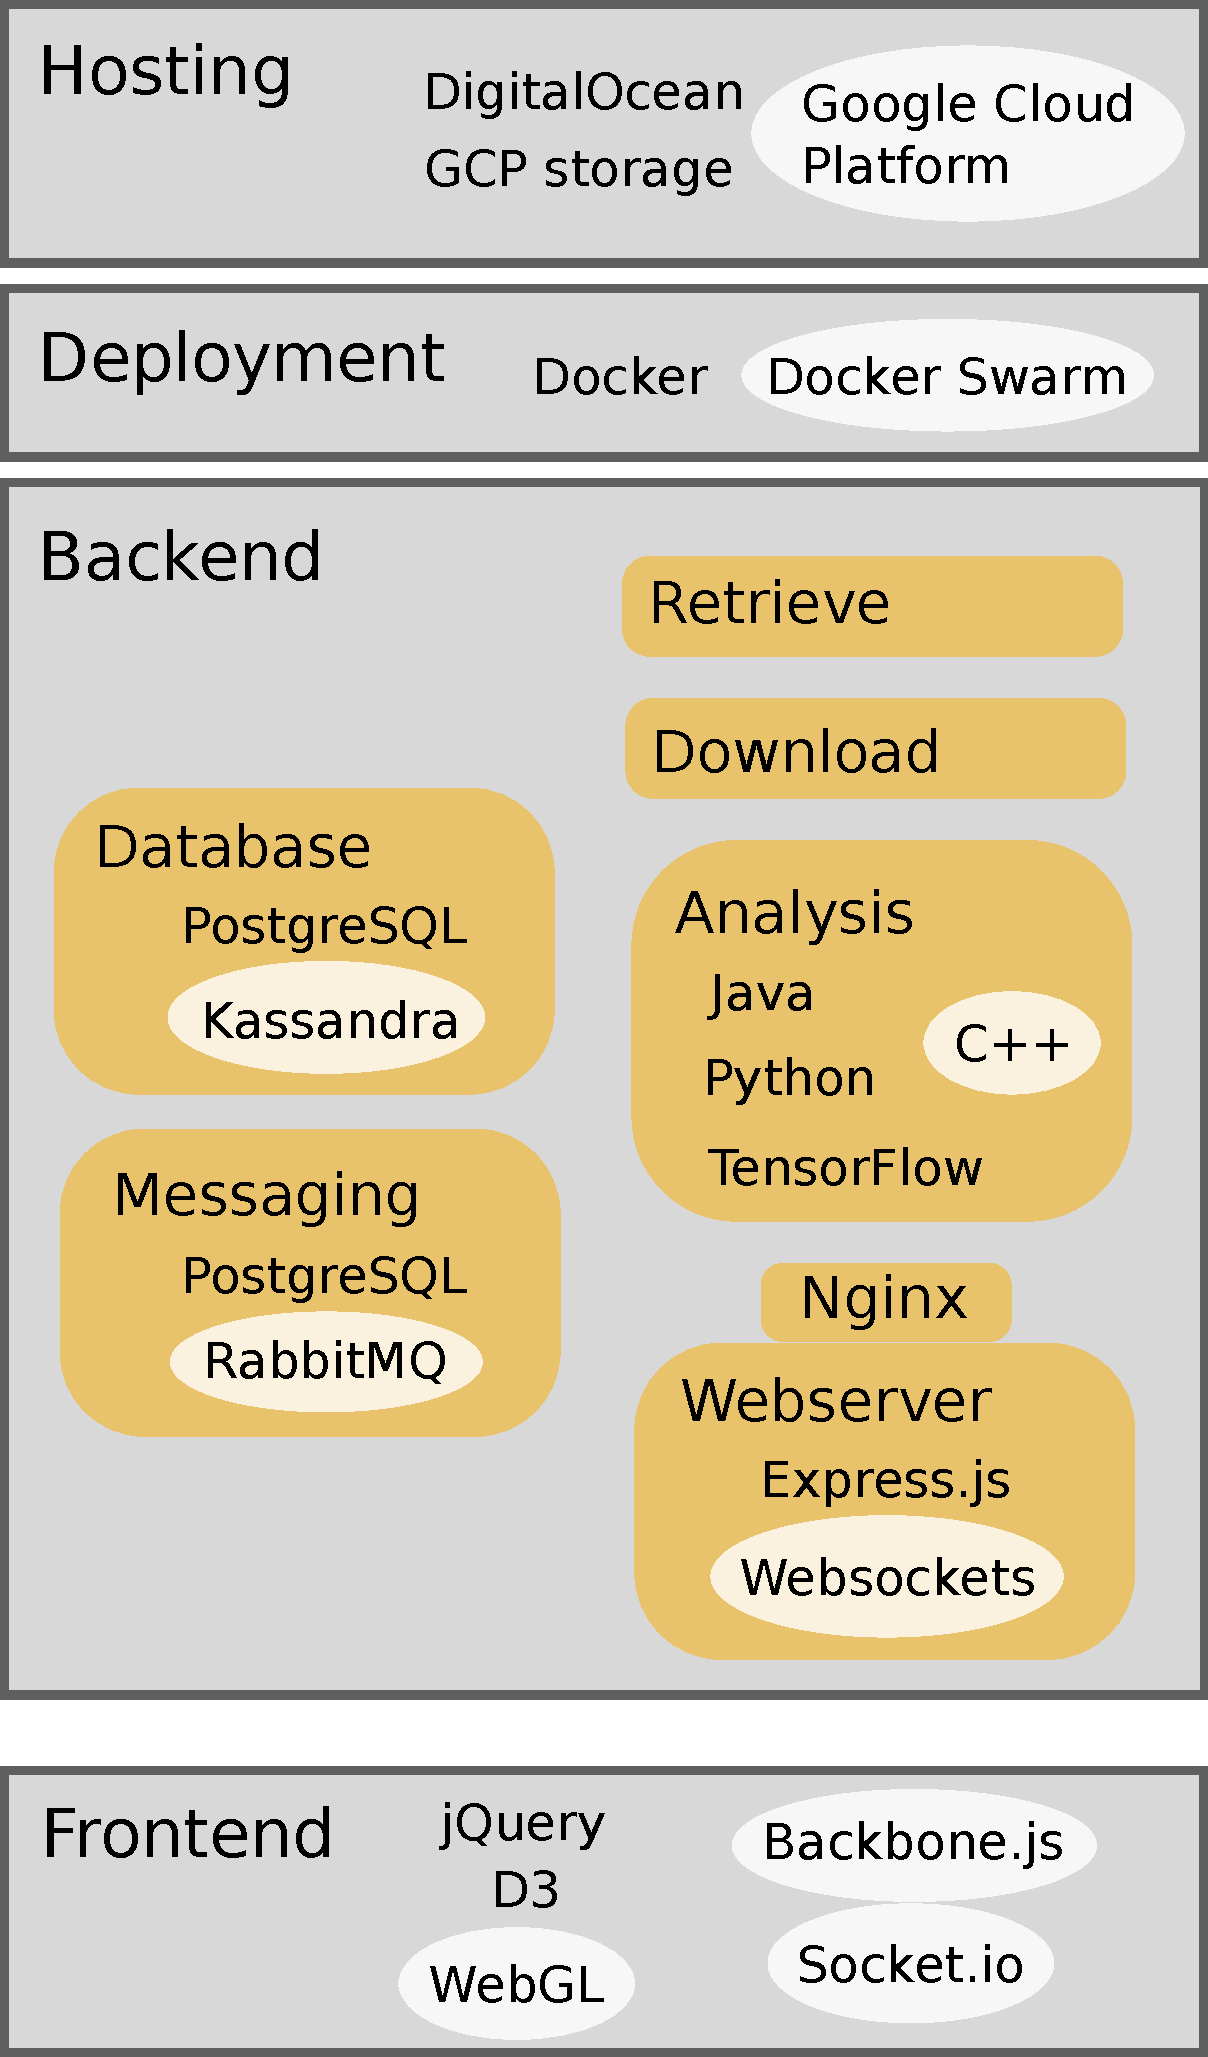
\includegraphics[width=0.9\textwidth,height=0.9\textheight,keepaspectratio]{img/diagram.pdf}
           \label{fig:tech-diagram}
           \caption{The technology stack of our webservice. Areas for future development are highlighted.}
\end{figure}

\section{Team}

\begin{description}
    \item [CEO] Continual customer development, hiring, and joint development of AI. Held accountable for the funnel and management of the team as a whole.
    \item [CTO] Architecture of the system, implementation of the production code for the platform and development of the AI. Held accountable for the performance of the entire tech stack.
    \vspace{0.5cm}
    \item [Frontend developer] Improvement of the UI and writing the HTML/CSS/JavaScript code for new features. Improving page load times by delivering data to user via web-sockets. Ideally would also have experience with D3.js. Potential candidates: Eugenio De Paulo, Daniel Seiler, Matei Rogoz.
    \item [Backend developer]  Improvement of the scalability of the back-end and transitioning to the GCP platform. Must have experience with Kubernetes, SQL, and configuring Linux servers.

    \item [Marketing Manager] Development of a marketing strategy, generation of content for the site and/or building partnerships with existing figures in the Dota community to publish content on Wisdota.com
    \item [Web designer(s)] Hired on a contract basis when new features are added to the site are required to be integrated into the existing design. Potential candidates: Klauss Andrei
\end{description}

\section{Timeline}

\subsection[Sep.-Dec. 2016 (Current State)]{September-December 2016 (Current State)}
\begin{itemize}
\item Main Objective: Raise money and find suitable hires
\item Team: 2 Cofounders 
\item Tasks:
\begin{itemize}
\item CEO: Raise funding and identify candidates to hire 
\item CTO: Begin transition towards new architecture on GCP.
\end{itemize}
\end{itemize}

\subsection[Jan.-June 2017 (Phase 1)]{January-June 2017 (Phase 1)}
\begin{itemize} 
\item Main Objective: Deliver first paid features.
\item Team: 2 Cofounders, Back-end Developer, Front-end Developer, (Web Designer on contract)
\item Tasks:
\begin{itemize} 
\item CEO: Customer development, managing team and developing AI
\item CTO: Event based summary of match based on segmentation of data set, automatic parsing for paying subscribers.
\item Backend developer: improving scalability of back-end
\item Frontend developer: improving UI and rate at which pages are served
\item UI/Web design contractor: Update match review design
\end{itemize}
\item Team Target: achieve 15k free users and 300 paying subscribers.
\end{itemize} 

\subsection[July-Dec. 2017 (Phase 2)]{July-December 2017 (Phase 2)}
\begin{itemize}
\item Main Objective: Develop more general AI tech and grow user base
\item Team: 2 Cofounders, Front-end developer, Back-end developer, Marketing Manager, (Web Designer on contract)
\item Tasks:
\begin{itemize}
\item CEO: Customer development and contributing to machine learning research.
\item CTO: Development of  machine learning/AI for recommending areas in which to improve play based on finding features that separate beginner/expert players and selecting optimal actions. 
\item Back-end developer: optimising code to reduce analysis time
\item Frontend developer: incorporating the new AI features into the front-end
\item Marketing Manager: Focusing on improving virality of the product and generating content for website.
\item UI/Web design contractor: Design of overlays for the automated coaching.
\end{itemize}
\item Team Target: 10-15\% monthly growth in users numbers, improvement in conversion rate from free to paid from 3\% to 5\%. Monthly churn rate of 10\% or lower.
\end{itemize}

\subsection[Jan.-June 2018 (Phase 3)]{January-June 2018 (Phase 3)}
\begin{itemize}
    \item Main Objective: Talking to investors to raise Series A and laying the groundwork to expand into other eSports (League of Legends, Counter-Strike). Development of video rendering capabilities,
\item Team:  2 Cofounders, Front-end developer, Back-end developer, Marketing Manager, (Web Ddesigner on contract)
\item Tasks:
\begin{itemize}
\item CEO: Sourcing of potential hires, building partnerships with developers, talks with investors to organise Series A.
\item CTO: Development of cloud video rendering system and software for capturing packets on client side.
\item Backend developer:  Implementation of parts of the video rendering backend
\item Frontend developer: Incorporation of the videos into the front-end
\item Marketing Manager: Focusing on building awareness and generating sign-ups for next products whilst continuing to create content for Dota project.
\item UI/Web design contractor: Design of landing page and signup page for League of Legends and Counter-Strike.
\end{itemize}
\item Team Target: 20-30\% monthly growth in users numbers, monthly churn rate of 10\% or lower and \pounds20k MRR from the Dota 2 product. Collection of at least 2000 emails per month for advanced access to the League of Legends and Counter-Strike products.
\end{itemize}

\subsection[{July 2018 - Future}]{July 2018 - Future}
\begin{itemize}
\item Main Objective: Expand into other eSports (League of Legends, Counter-Strike) and provide game developers with an easy to integrate layer that helps them monetise coaching in their games.
\begin{samepage}
\item Team (14 in total):  
\begin{itemize}
\item (2) Cofounders, 
\item (7) Engineering: Dev ops, Front-end developer, Back-end developer, League Lead developer, League Junior developer, CS:GO Lead developer, CS:GO Junior developer
\item (2) Research Team: 2 x AI researchers
\item (2) Marketing: Marketing Manager, Junior Marketer
\item (1) Business Development: Business Development Manager
\end{itemize}
\end{samepage}
\end{itemize}

\subsection{Vision in 5 Years} 
We are the category leader for AI coaching for 4-5 of the major eSports titles. We have expanded first to League of Legends, then CS:GO, world of tanks etc. giving us an audience close to 100M players. We've partnered with top eSports teams and the analysis is regularly used live in major tournaments. The technology in the back end is general enough to plug new games into in the space of weeks/months. We are recognised as developers of new and innovative AI methods.

\section{Market Analysis}
 
In this section we consider three categories of products that eSports players currently use to improve their play, and then give a brief overview of two other startups competing in the same space.
 
\subsection{Video Platforms}
 
Over a hundred million people watch games being played online each month via video platforms such as Twitch and Youtube. One of the major motivations for watching eSports is to learn how to get better at playing by watching expert players \cite{Hamari15}. Our hypothesis is that there exists a large subset of viewers who watch Twitch and Youtube videos on eSports specifically in order to learn how to improve, but are underserved by the present offerings because the content that video platforms provide cannot be tailored to coach individual players.\\
 
The eSports video platform market is dominated by Twich.tv and Youtube's gaming channel. Twitch.tv is a live video platform and community for gamers with more than 100 million unique users per month and was acquired by Amazon for \$970M cash after three years of development. Twitch boasts a highly engaged audience, with the average user watching 1.5 hours of videos per day \cite{Dredge}. Youtube is the well-known video sharing website, with a broad range of video categories. It recently added live streams to compete with Twitch, and games have become the No.1 category on Youtube in terms of viewership.
 
\subsection{Game Statistics Websites}
 
Statistics websites such as Dotabuff.com and Yasp.co are is widely used by eSports players who wish to improve their play. These websites provide tables of statistics from eSports matches on specific aspects of the game, such as how much gold an individual has earned per minute or how many fights they were involved in.

\begin{description}
    \item [Dotabuff.com] features tables of statistics as well as articles and forums, and has over a million users. Dotabuff monetises the content through two channels: advertising, and a premium service, which grants subscribers access to more in depth statistics for the cost of \$6 per month or \$56 per year. Dotabuff uses its own hardware for the computation.
 
    \item [Yasp.co] is a not-for-profit website developed by members of the Dota community and is funded via donations from users. Yasp parses replay files and calculates tables of statistics, duplicating much of the functionality of Dotabuff.com. The site has 85k signed in users, of which 26k used the site in the past two weeks. Yasp uses 15+ rented servers to parse 30k games per day.
\end{description}

\subsection{One-to-one Coaching Websites }
 
A third category of products that eSports players currently use to improve their play is one-to-one coaching websites. These websites typically function as a platform where users can select coaches from a list of profiles that display the price per hour and some metric of experience. Using a messaging service the user can contact the coach and organise a time to have the lesson.
 
For example, Lol-coaching.com is a one-to-one coaching platform for League of Legends and claims 40k students and 17k coaches. The company charges a 15\% fee to handle payments for lessons (though the payments themselves are handled by PayPal). Dotacoach.org is a similar platform but for Dota 2, with 200 registered coaches.

\subsection{Direct Competitors}

\begin{description}
 \item [Dojo Madness (www.dojomadness.com)] Berlin based startup founded by Jens Hilgers, currently has approximately 20 employees. Plan to apply machine learning and big data techniques to help players improve at their game. Focussed for the time being on mobile apps that function as second screens whilst you play. They have a product called LolSumo which provides basic tips whilst playing League of Legends - decent traction with 70k DAU. Recently raised \$4.5m seed round.

 \item [Eblur (www.eblur.co.uk)] Part of the EF6 cohort, initially planned to build a video clips site for eSports, but then switched to also build an AI coach for Dota. Plan to provide the coaching in real time by scraping pixels from the user's screen. Their product requires users to download software to the do the analysis on their PC. Have struggled to gain users as Dota players fear they may be banned by the game's developer for using the software (see Reddit thread: \cite{Eblur}).
\end{description}

\subsection{Comparison with Tembryo}
 
Our platform will provide three main advantages over existing one-to-one coaching solutions: 
\begin{description}
    \item [Quality] Our platform will make use AI and a large data set of replay files to provide tips to users that are grounded in data, for example ``taking action X leads to 65\% win rate'', as compared to subjective advice from a live coach.
    \item [Price] By automating the process we are able to provide the service at \$5-10 per month compared to \$10-25 per hour.
    \item [Convenience] Users don't have to schedule lessons in advance as they would with a live coach. They can get tips whenever they want, in as much detail as they want.
\end{description}

DojoMadness has - after one tech demo two years ago - not shown progress at building products for Dota 2 and confirmed in talks earlier this year that their team is busy developing the existing apps for League of Legends. They also have expressed their preference for a different approch to game analysis, which involves crowdsourcing human players' analysis instead of AI optimisation, which we believe to be inferior.

Our main advantage over Eblur (and partly DojoMadness) is that the technology we have developeddoes not require the user to not have to install any additional software. In addition the Eblur approach of inferring the game state from pixels on the user's screen adds another layer of technical difficulty to the problem of building an AI coach, and so far has limited them to providing basic insights based on the 2D minimap on the Dota screen, it is not clear how they plan to go beyond this to interpreting 3D scenes. 

\begin{thebibliography}{10}

\bibitem{Hamari15}  Hamari  {\em What is eSports and Why Do People Watch It?} 2015. Available at \url{http://ssrn.com/abstract=2686182}.
\bibitem{Eblur} Reddit \url{https://www.reddit.com/r/DotA2/comments/4snuhi/anyone_tried_feedless_from_eblur_ai/}.
\bibitem{Dredge} Dredge  {\em Youtube v Twitch: battling for viewers, but both can grow}  2015. Available at: \url{http://www.theguardian.com/technology/2015/sep/28/twitch-youtube-live-streaming-amazon-gaming-audience}.

\end{thebibliography}

\end{document}